\begin{savequote}[45mm]
\ascii{Any fool can write code that a computer can understand. Good programmers write code that humans can understand.}
\qauthor{\ascii{- Martin Flower}}
\end{savequote}

\chapter{破冰之旅} 
\label{ch:ice-breaker}

\begin{content}

\end{content}

\section{编程环境}

\begin{content}

\subsection{系统配置}

\begin{colortable}{X|X|X}{环境配置}
\emph{名称}                      & \emph{配置}          & \emph{版本}      \\\hline
\multirow{2}{*}\ascii{操作系统}  & \ascii{Linux Kernel} & \ascii{4.15.0}  \\\cline{2-3}
                                & \ascii{Ubuntu}       & \ascii{18.04}   \\\hline
\multirow{2}{*}\ascii{编译器}    & \ascii{GCC}          & \ascii{7.3.0}   \\\cline{2-3}
                                & \ascii{Clang}        & \ascii{6.0.0}   \\\hline
\ascii{编程语言} & \ascii{C++}   & \ascii{14}                              \\\hline
\multirow{2}{*}\ascii{构建工具}  & \ascii{CMake}        & \ascii{3.10}     \\\cline{2-3} 
                                & \ascii{Make}         & \ascii{4.10}     \\\hline
\ascii{集成开发环境}              & \ascii{Eclipse CDT}  & \ascii{Oxygen 3} \\\hline 
\ascii{版本工具}                 & \ascii{Git}          & \ascii{2.17.1}   \\\hline
\end{colortable}

\subsection{项目组织}

\ascii{xUnit Mars}项目目录结构如\refig{mars-project}所示。

\begin{figure}[H]
\centering
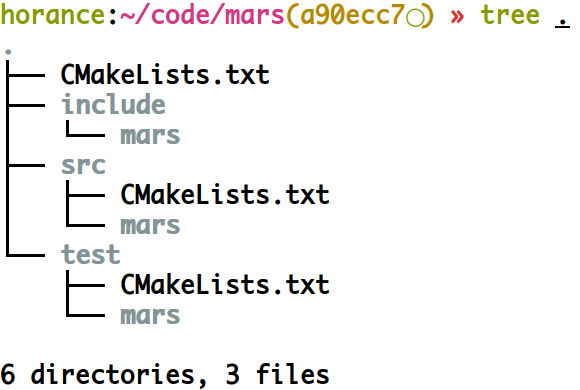
\includegraphics[width=0.6\textwidth]{figures/xunit/mars-project.png}
\caption{xUnit Mars: 项目组织}
 \label{fig:mars-project}
\end{figure}

\begin{episode}{代码风格}

\begin{content}

\emph{团队成员遵循\ascii{XP}基本价值观,致力于优秀的软件设计。}系统中所有的代码看起来就好像是由单独一个值得胜任的人编写的,并遵循一致的、统一的的代码风格。

可以配置\ascii{Eclipse CDT}代码模板,团队通过导入代码模板,使其得到一致的代码风格。业界存在多种经典的代码风格,团队应该选择并保持其中一种代码风格。

\begin{enum}
  \eitem{\code{K\&R}}
  \eitem{\code{BSD/Allman}}
  \eitem{\code{GNU}}
  \eitem{\code{Whitesmiths}}
\end{enum}

本书使用\ascii{K\&R}的代码风格,但在对齐方面做了细微调整,如\refig{eclipse-formatter}所示。配置完毕之后,便可以充分享受神奇带来的快感。

例如,创建头文件时,自动生成\ascii{UUID}的头文件保护宏,彻底抛弃这个遗留问题;当需要排版代码时,使用快捷键\ascii{Ctrl + Shift + F}立马得到漂亮的代码风格。

关于\ascii{Eclipse CDT}详细配置与使用技巧,推荐阅读王博\footnote{\href{https://www.jianshu.com/u/92b7d9879f20}{\ascii{https://www.jianshu.com/u/92b7d9879f20}}}在简书上的三篇博文:\href{https://www.jianshu.com/p/dafcdce1f9cb}{\ascii{Effective Eclipse CDT}}。

\begin{figure}[H]
\centering
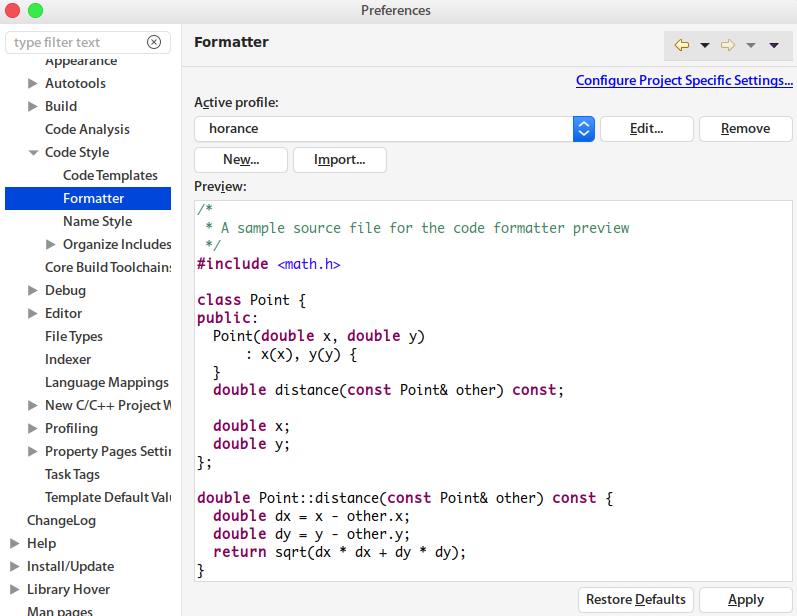
\includegraphics[width=1.0\textwidth]{figures/xunit/eclipse-formatter.png}
\caption{代码风格: K\&R}
 \label{fig:eclipse-formatter}
\end{figure}

\end{content}

\end{episode}

\subsection{构建系统}

\ascii{xUnit Mars}使用\ascii{CMake}构建工具。在项目根目录下,主控\ascii{CMakeLists.txt}完成项目的整体配置,及其子任务的组织。

\begin{nodiff}{CMakeLists.txt}
 \begin{c++}
project(mars)                                                                                  
cmake_minimum_required(VERSION 2.8)

set(CMAKE_CXX_FLAGS "${CMAKE_CXX_FLAGS} -std=c++14")

include_directories("${CMAKE_CURRENT_SOURCE_DIR}/include")

add_subdirectory(src)
add_subdirectory(test)
 \end{c++}
\end{nodiff}

\ascii{src/CMakeLists.txt}完成\ascii{mars}库构建。

\begin{nodiff}{src/CMakeLists.txt}
 \begin{c++}
file(GLOB_RECURSE all_files *.cc)
add_library(mars STATIC ${all_files})
 \end{c++}
\end{nodiff}

\ascii{test/CMakeLists.txt}完成\ascii{mars-test}应用程序构建,它执行\ascii{xUnit Mars}项目的所有测试用例。

\begin{nodiff}{test/CMakeLists.txt}
 \begin{c++}
file(GLOB_RECURSE all_files *.cc)
add_executable(mars-test ${all_files})
target_link_libraries(mars-test mars gtest gtest_main pthread)
 \end{c++}
\end{nodiff}

\subsection{Git库}

在项目根目录下初始化一个空的\ascii{Git}库。

\begin{nodiff}{初始化git库}
 \begin{c++}
$ git init
 \end{c++}
\end{nodiff}  

待项目组织完毕,完成第一次代码提交。

\begin{nodiff}{提交代码}
 \begin{c++}
$ git add -A .
$ git commit -m"setup project"
 \end{c++}
\end{nodiff}

\end{content}

\section{起航}

\begin{content}

\subsection{测试用例}

万事开头难,第一个用例跑起来并不容易。此处设计实现了一个简单的测试用例,用户通过扩展\ascii{xUnit Mars}框架中的\ascii{TestCase},实现测试用例的增加。

\begin{nodiff}{test/mars/core/TestCaseSpec.cc}
 \begin{c++}
#include <gtest/gtest.h>
#include "mars/core/TestCase.h"

namespace {
  struct SimpleTest : TestCase {
    bool wasRun = false;

  private:
    void run() override {
      wasRun = true;
    }
  };

  void run(TestCase& test) {
    test.run();
  }
}

TEST(SimpleTest, make_sure_test_case_can_run_normally) {
  SimpleTest test;
  run(test);

  ASSERT_TRUE(test.wasRun);
}
 \end{c++}
\end{nodiff}

\begin{episode}{TDD: 测试驱动开发}

\begin{content}

\ascii{TDD}是极限编程中重要的技术实践之一。\ascii{TDD}遵循\emph{测试先行,小步快走,尽快变绿,事后重构}的基本方法论。把握\ascii{TDD}动态变化过程,做到收放自如,需要长期编程实践的经验积累。

\ascii{TDD}基本素养讲究两个字:“小”和“快”。“小”体现在测试刚好失败,实现恰如其分,重构步骤粒度甚微。而“快”体现不在于编程速度,而在于“尽最小努力,最短时间,最快通过测试”。

如果步子迈得过大,则恢复测试时间间隔会变长,信心指数则会下降,自然影响软件质量,甚至拖延软件交付进度。

\subsubsection{TDD闭环}

如\refig{tdd-cycle}所示,在一轮\ascii{TDD}编程实践过程中,遵循三部曲的闭环操作:\ascii{“Red-Green-Refactor”}。每轮迭代之后,确保系统都处于一个相对合理的状态。

\begin{figure}[H]
\centering
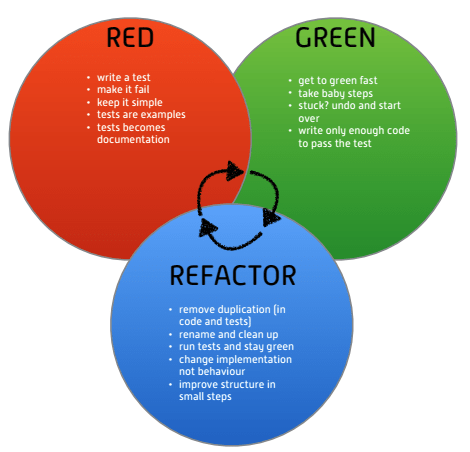
\includegraphics[width=0.8\textwidth]{figures/xunit/tdd-cycle.png}
\caption{TDD: 测试驱动开发}
 \label{fig:tdd-cycle}
\end{figure}

\subsubsection{TDD实现方法}

极限编程之父\ascii{Kent Beck}在经典著作\ascii{Test-Driven Development by Example}之中,介绍了三种基本的实现方法。

\begin{enum}
  \eitem{伪实现}
  \eitem{三角法}
  \eitem{显式实现}
\end{enum}

使用硬编码,伪装通过测试是一种最快速、最简单的实现方法。一旦通过测试,然后通过重构消除重复,以期待消除所有硬编码;或使用三角法,添加新的测试用例,驱动真实实现。

除非问题看起来并没有想象中那么简单,可以采取保守的策略也是恰当的。如果实现显而易见,完全可以绕开保守的\emph{伪实现}与\emph{三角法}。而在实际操作中,通过测试往往都比较简单,显式实现也是最常见的做法。在这种情况下,大可快速前进,不用处处敬小慎微。

\subsubsection{尽快变绿}

三种实现方法常常交替使用,虽然实现迥异,但殊途同归:以最小的努力,在最短的时间,通过测试,尽快变绿。实现过程中,尽量不要引入过度复杂的实现。例如,引入某种设计模式,重构既有的代码。

务必克服心中的恶魔,需要充分衡量成本收益比。如果引入设计较为笨重,通过测试遥遥无期,则应立即放弃;而如果引入设计显而易见,实施起来也比较容易操作,并带来一定设计的弹性,且不影响通过测试的整体进度,则可以有限接受。

\subsubsection{重构成为习惯}

一旦测试通过,务必重构既有的实现,让设计保持在目前最合理的状态。此刻,也需要克服心中的恶魔,不能做过度的设计。如果没有测试用例表达某个事件发生,则不要凭空臆想未来的世界会发生什么事情。

\subsubsection{出错后放慢脚步}

在最坏的情况下,测试在一段时间内尝试修复都以失败告终,则需要使用\ascii{Git}回退所有代码,使用更保守的\emph{伪实现}与\emph{三角法},尽快修复测试。

\subsubsection{TDD实现原则}

\ascii{Bob}大叔在其著作\ascii{Clean Code}中阐述了实践\ascii{TDD}的三个基本原则。

\begin{enum}
  \eitem{在编写不能通过的测试前,不可编写生产代码;}
  \eitem{只可编写刚好无法通过的测试,不能编译也算不通过;}
  \eitem{只可编写刚好足以通过当前失败测试的生产代码。}
\end{enum}

理解起来比较绕口,换一个等价的、较易理解的方式,可以表述为:

\begin{enum}
  \eitem{测试先行;}
  \eitem{测试失败;}
  \eitem{尽快变绿。}
\end{enum}

\subsubsection{TDD实现技巧}

实践\ascii{TDD}时,常需要规划和维护一个\ascii{TODO List}。将熟悉的,价值大,容易实现,高优先级的测试用例优先实现;而将不熟悉,价值小,不易实现,异常边界的测试用例依次排到后面,留待后续处理。

\begin{enum}
  \eitem{基本功能与异常场景;}  
  \eitem{高价值与现成果实;}
  \eitem{确定与不确定;}
  \eitem{整体优先与细节优先。}
\end{enum}

\end{content}

\end{episode}

\subsection{通过编译}

此处引入了多态技术,当\ascii{TestCase::run}启动运行时,将在运行时调用覆写的\ascii{SimpleTest::run},实现自定义测试用例的执行。

\begin{nodiff}{include/mars/core/TestCase.h}
 \begin{c++}
#ifndef H586108AA_CD7B_459D_8A2F_0DFE6C9720ED
#define H586108AA_CD7B_459D_8A2F_0DFE6C9720ED

struct TestCase {
  virtual void run() = 0;
  virtual ~TestCase() {}
};

#endif
  \end{c++}
\end{nodiff}

\begin{episode}{头文件保护宏}

\begin{content}

\ascii{C/C++}编译模型通过使用\ascii{include}语句导入头文件而实现的。为了避免头文件被导入多次,每一个头文件都应该定义独一无二的头文件保护宏。社区存在两种典型的代码风格:

\begin{enum}
  \eitem{\code{INCL\_<PROJECT>\_<MODULE>\_<FILE>\_H}}
  \eitem{\code{UUID}}
\end{enum}

第一种命名风格问题在于:当头文件被重命名或移动目录时,为了保持一致性需要同步修改头文件保护宏,而此特性\ascii{IDE}通常支持都不是太良好。因此,推荐随机生成\ascii{UUID},其更加快捷、简单、并且安全、有效。

首先,配置\ascii{Eclipse CDT}的代码模板。当创建头文件时,自动生成头文件保护宏。

\begin{figure}[H]
\centering
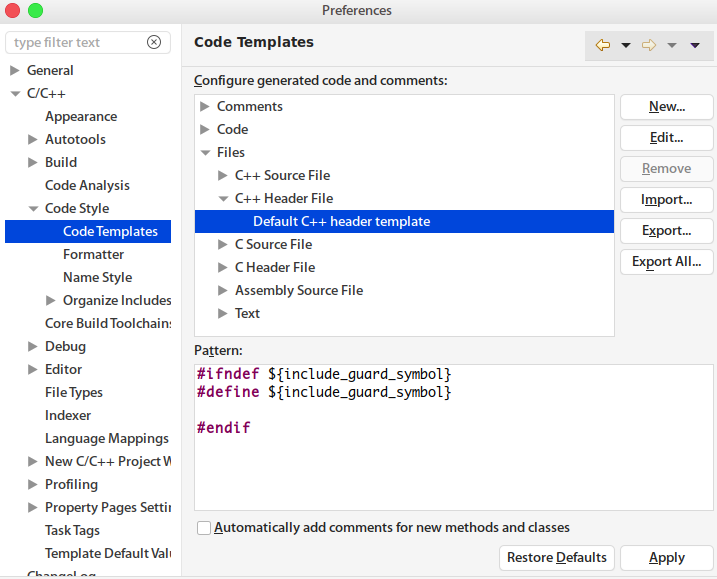
\includegraphics[width=0.95\textwidth]{figures/xunit/eclipse-code-template.png}
\caption{Eclipse CDT: 代码模板}
 \label{fig:eclipse-code-template}
\end{figure}

然后,配置头文件保护宏使用\ascii{UUID}自动生成。

\begin{figure}[H]
\centering
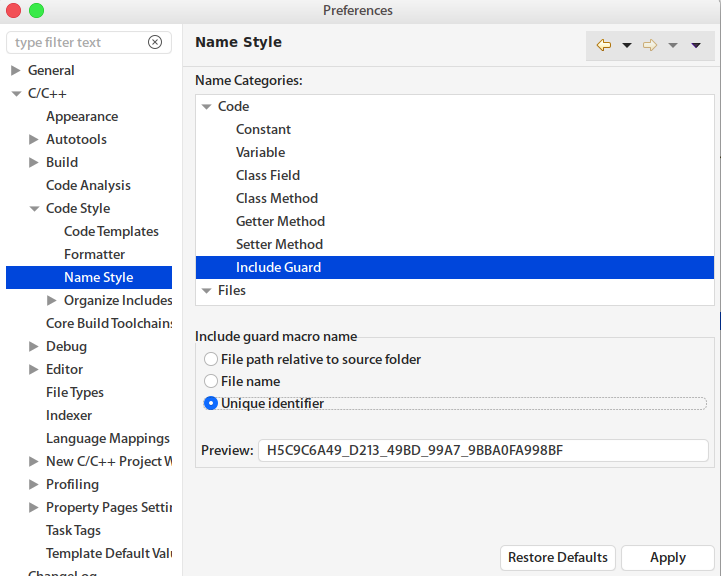
\includegraphics[width=0.95\textwidth]{figures/xunit/eclipse-include-guard.png}
\caption{Eclipse CDT: 生成UUID的头文件保护宏}
 \label{fig:eclipse-include-guard}
\end{figure}

为了缩短篇幅,后文略去所有头文件保护符。

\end{content}
\end{episode}

需要关注的是,\ascii{TestCase}实现了一个虚拟析构函数。如果不经意地遗忘声明该析构函数为虚拟的\footnote{默认生成的析构函数是公开的、非虚拟的、内联实现的。},则可能招致运行时不确定的行为发生。

\begin{episode}{虚拟析构函数}
\begin{content}

一般地,需要为\emph{多态基类}声明虚拟析构函数;否则,会招致运行时不可预期的行为。一般地,如果一个类包含虚函数时,便将其析构函数声明为虚拟的。

\subsubsection{空实现}

但是,为每个接口类型实现一个空的虚拟析构函数,显得重复而且麻烦。可以引入一个宏定义,自动引入空实现的虚拟析构函数。

 \begin{c++}
namespace details {
  template<typename T>
  struct Trait {
    virtual ~Trait() {}
  };
}

#define TRAIT(trait)  struct trait : ::details::Trait<trait>
#define EXTENDS(...) , ##__VA_ARGS__
 \end{c++}

例如,使用\ascii{TRAIT}宏,定义了一个接口类型\ascii{SelfDescribing},它自动拥有虚拟析构函数的默认空实现。

 \begin{c++}
struct Description;

TRAIT(SelfDescribing) {
  virtual void describeTo(Description& desc) const = 0;
};
 \end{c++}

\subsubsection{抽象函数}

此外,定义纯虚函数时,常常会遗忘后面的\ascii{0}。可以引入另外一个宏定义。

 \begin{c++}
#define ABSTRACT(...) virtual __VA_ARGS__ = 0
 \end{c++}

使用\ascii{ABSTRACT}定义,不仅可以抑制不经意地遗漏\ascii{0}的错误,也可以改善\ascii{API}的意图和可读性。

\begin{c++}
struct Description;

TRAIT(SelfDescribing) {
  ABSTRACT(void describeTo(Description& desc) const);
};
\end{c++}

\end{content}
\end{episode}

\subsection{通过链接}

创建一个空的\ascii{TestCase.cc}文件,这里仅为了\ascii{libmars.a}不为空,保证\ascii{CMake}构建系统工作正常;否则,\ascii{CMake}提示\ascii{mars}项目为空,无法构建\ascii{libmars.a}库。

\begin{nodiff}{src/mars/core/TestCase.cc}
 \begin{c++}
#include "mars/core/TestCase.h"
 \end{c++}
\end{nodiff}

\begin{episode}{多屏编辑}

\begin{content}

在\cpp{}编程实践中,需要在头文件和实现文件之间频繁切换。同时,在\ascii{TDD}编程实践中,也需要在测试文件与头文件/实现文件之间频繁切换。

得益于现代\ascii{IDE}的丰富特性,推荐多屏显示相关源文件。例如,如\refig{multi-editor-eclipse}所示,使用\ascii{Eclipse CDT},三屏分别显示相关联的头文件、实现文件,及其测试用例文件。

\begin{figure}[H]
\centering
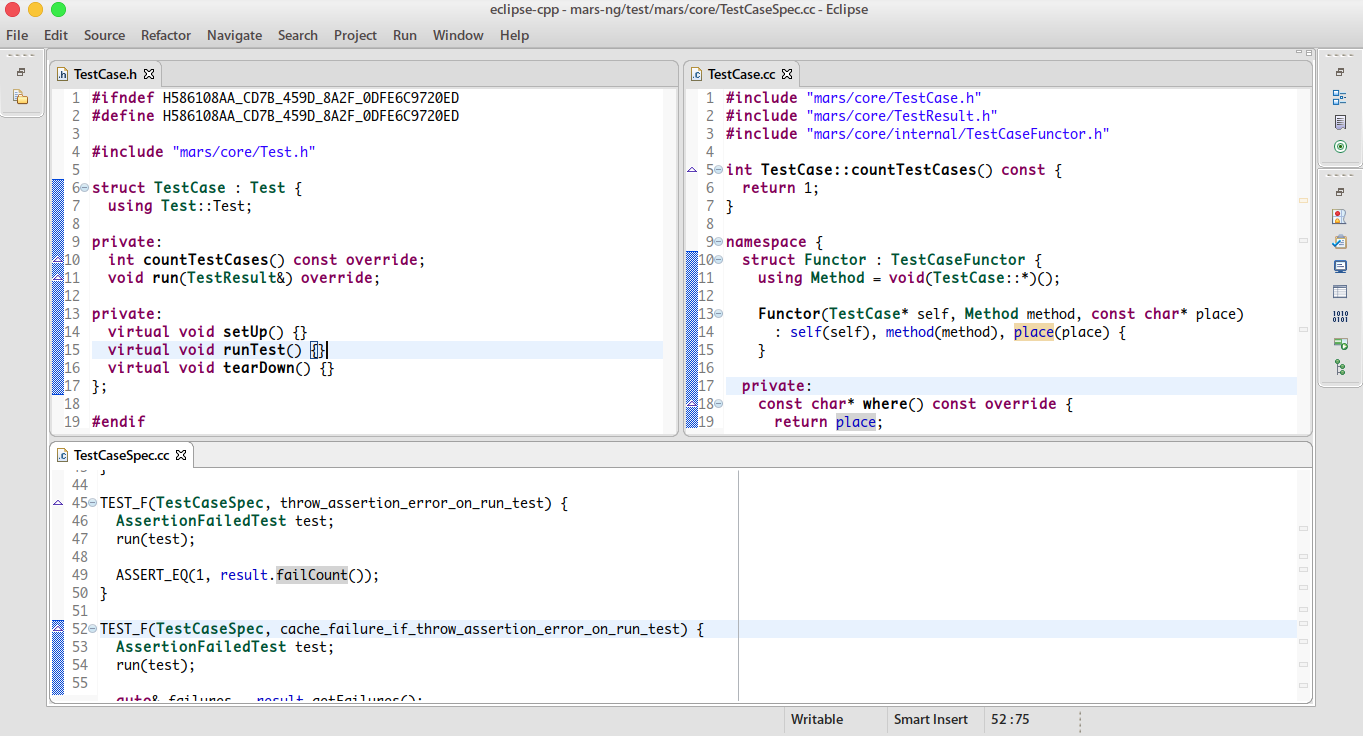
\includegraphics[width=1.0\textwidth]{figures/xunit/multi-editor-eclipse.png}
\caption{Eclipse CDT: 多屏显示}
 \label{fig:multi-editor-eclipse}
\end{figure}

推荐购置高清,大屏显示器,有效改善编程环境,从而提高工作效率。关闭无关的\ascii{Tab}页,只打开当前相关的文件,最小化外部干扰;一则让\ascii{IDE}运行速度最佳,二则使用诸如\ascii{Ctrl + E}快捷键切换文件时,最小化文件列表长度。

强烈推荐使用快捷键的优秀实践,可以成倍地提高编程的效率。例如,使用快捷键\ascii{Ctrl + Tab},在头文件与实现文件间切换自如。

\end{content}

\end{episode}

\subsection{通过测试}

在\ascii{build}临时目录中,使用\ascii{cmake}构建工程。

\begin{nodiff}{构建工程}
 \begin{c++}
$ mkdir -p build && cd build
$ cmake ..
$ make
 \end{c++}
\end{nodiff}

运行测试。

\begin{nodiff}{运行测试}
 \begin{c++}
$ test/mars-test
Running main() from gtest_main.cc
[==========] Running 1 test from 1 test case.
[----------] Global test environment set-up.
[----------] 1 test from SimpleTest
[ RUN      ] SimpleTest.make_sure_test_case_can_run_normally
[       OK ] SimpleTest.make_sure_test_case_can_run_normally (0 ms)
[----------] 1 test from SimpleTest (0 ms total)

[----------] Global test environment tear-down
[==========] 1 test from 1 test case ran. (0 ms total)
[  PASSED  ] 1 test.
 \end{c++}
\end{nodiff}



\begin{episode}{全局忽略模式}

\begin{content}

\ascii{CMake}在临时目录\ascii{build}中完成系统构建,为了避免不经意地将\ascii{build}目录提交至\ascii{Git}库,常常需要在\ascii{.gitignore}文件中配置相应的忽略模式。

但是,为每个项目都创建一个\ascii{.gitignore}文件,显然是一种重复设计。因此,配置全局忽略模式是一个更恰当的解决方案。

 \begin{c++}
$ git config --global core.excludesfile ~/.gitignore_global
$ vi ~/.gitignore_global
# cmake
build/

# vi
*.swp

# eclipse
.project
.cproject
.settings/

# tex
output/
 \end{c++}

\end{content}
\end{episode}

\subsection{提交代码}

每当通过测试后,立即提交代码到\ascii{Git}库。

\begin{nodiff}{提交代码}
 \begin{c++}
$ git add -A .
$ git commit -m"pass first test case"
 \end{c++}
\end{nodiff}

\begin{episode}{后悔药}

\begin{content}

感谢\ascii{Linus}创造了\ascii{Linux}与\ascii{Git},让全世界的程序员得以享受编程的快乐。\ascii{TDD}精髓之一便是“小”,配合运用\ascii{Git},简直就是完美,避免不经意的错误而丢失代码。

养成经常性提交代码至\ascii{Git}库,是一种良好的编程习惯。在\ascii{TDD}的一个迭代循环中,每当编译通过,链接通过,测试通过,关键重构成功,都应立即执行\ascii{git add}。当设计重构至相对合理状态,最后执行\ascii{git commit}入库,完成一次\ascii{TDD}的闭环。

此外,借助于\ascii{Git},随时可以吃后悔药。当尝试某种重构设计时,没有达到预期效果,则可以轻松回到上一个稳定状态,重新开始尝试新的努力。以“重命名函数”的重构过程为例,讲述\ascii{Git}的操作。

\begin{enum}
  \eitem{新建一个函数;}
  \eitem{拷贝旧函数的实现至新函数;}
  \eitem{确保编译、测试通过,执行\code{git add};}  
  \eitem{删除旧函数的实现逻辑,转调新函数;}
  \eitem{确保编译、测试通过,执行\code{git add};}
  \eitem{对于每个引用旧函数的地方,重构引用新函数,确保编译、测试通过,执行\code{git add};}    
  \eitem{删除旧函数,确保编译、测试通过,执行\code{git commit}。}      
\end{enum}

\end{content}
\end{episode}

\end{content}

